\label{sec:4}

Both the automatic parallelisation compiler and Kautuka's language design \textbf{exceed the project's core success criteria}. In section \hyperref[sec:4.1]{4.1}, I demonstrate how the project achieves all core criteria set out in the project proposal (appendix \hyperref[sec:F]{F}). I then evaluate the project beyond the original success criteria using my three research questions (listed below) as a basis. Sections \hyperref[sec:4.2]{4.2} to \hyperref[sec:4.4]{4.4} show that all three investigations yield \textbf{positive results}.

\vspace{1mm}

Research questions:
\vspace{-5mm}

\begin{enumerate}
  \setlength{\itemsep}{2pt}
        \setlength{\parskip}{0pt}
        \setlength{\parsep}{0pt}
  \item Transfer automatic-parallelisation theory from functional to imperative languages
  \item Investigate the performance of task-based parallelisation on I/O-bound programs
  \item Investigate real-world applications of the compiler
\end{enumerate}

\vspace{-3mm}

\section{Review of Project Requirements}

\label{sec:4.1}

Reviewing the feature requirements outlined in the preparation chapter (section \hyperref[sec:2.7.1]{2.7.1}), I implemented all \textit{Must-have} core deliverables and the majority of \textit{Should-have} and \textit{Could-have} extensions. Evaluating the project against the original success criteria from the project proposal (appendix \hyperref[sec:F]{F}) yields:

\begin{itemize}[itemindent=-1cm]
  \item[] \textbf{Design a full-featured imperative language Kautuka with a compiler to Go} I realised that creating a \textit{full-featured} programming language was not appropriate for a project of this size. So I constrained the project's scope to a \textit{mid-featured} language, with key features listed in the MoSCoW analysis of section \hyperref[sec:2.7.1]{2.7.1}. I completed all core and extension features from this table, excluding the \textit{Could-have} feature: recursion.
  \item[] \textbf{Implement side-effect tracking} The compiler successfully performs side-effect tracking with all proposed extensions: file I/O (with aliasing analysis) and console I/O (section \hyperref[sec:3.4]{3.4}).
  \item[] \textbf{Implement cost analysis} The compiler successfully implements type-cost analysis and runtime-cost analysis. I extended type-cost analysis with a powerful inference algorithm to minimise programmer effort. Section \hyperref[sec:4.2]{4.2} shows that runtime-cost estimates are sufficiently accurate to guide parallelisation.
  \item[] \textbf{Parallelise code based upon this analysis} Section \hyperref[sec:3.6]{3.6} describes how side-effect tracking and cost analysis influence parallelisation. The following success criteria analyses the efficacy of our approach.
  \item[] \textbf{Ensure that the produced parallel code is both \textit{safe} and \textit{efficient}} I provide empirical evidence for \textit{safety} through testing, performing a total of \textbf{48 tests} (section \hyperref[sec:4.2]{4.2}). To show that parallel code is \textit{efficient}, I benchmarked Kautuka against the equivalent sequential Go code. Section \hyperref[sec:4.3]{4.3} shows that Kautuka's performance \textit{exceeds} that of sequential Go for I/O-bound programs by an average of \( 35\% \).

\end{itemize}


\section{Functional to Imperative Theory}

\label{sec:4.2}

The core of high-level automatic parallelisation lies in side-effect tracking and cost analysis. While such techniques have been previously explored in the context of functional languages, implementing this theory into an imperative language compiler poses new challenges. This section evaluates the success of my solutions to these problems --- defined here as preserving the \textit{safety} of side-effect tracking and \textit{accuracy} of cost analysis.

I provide empirical evidence for side-effect tracking \textit{safety} through testing. I validate the correctness of each typing rule implementation with \textit{unit tests}, writing \textbf{38 tests} to cover all top-level expression constructions. To verify that safety extrapolates to more complex expressions, I implemented \textbf{10 component tests} --- testing edge cases between typing rule interactions. I translated ten non-trivial Go programs into Kautuka by hand, to produce a test corpus of Kautuka programs. These programs form the basis of my component testing, which validates the correctness of side-effect sets produced by each code block. To further substantiate claims of safety, I compared Kautuka's execution behaviour against the original Go code (repeating experiments to account for non-determinism). If these behaviours are identical, then I conclude that parallel code derived from Kautuka is \textit{race-free}.

\textbf{Results} All 38 unit tests and 10 component tests passed, and Kautuka's execution behaviour was identical to Go. These are promising results, suggesting that side-effect tracking is \textit{safe} and the produced parallel Go code is \textit{race-free}. However, it is impossible to construct a program corpus covering all edge cases; a way to guarantee safety would be through a formal proof.

The purpose of cost analysis (in this project) is to estimate program runtime. It is sufficient in our case to predict runtimes of the correct \textit{order of magnitude}. Hence, cost analysis is \textit{successful} if our predictions are within one order of magnitude (base 10) of the actual runtime. We use the corpus of Kautuka programs, mentioned previously, to compare \textit{predicted} and \textit{actual runtimes}.

\pgfplotstableread[row sep=\\,col sep=&]{
  input_param & actual & predicted & actual_order_plus & actual_order_minus  \\
  \texttt{fact} & 2534.326 & 6744.697 & 22808.934 & 2280.893 \\
  \texttt{sum\_factors} & 604.505 & 2449.218 & 5440.545 & 544.054 \\
  \texttt{parse\_files} & 2886.866  & 1382.430  & 25981.794 & 2598.179 \\
  \texttt{generate\_files} & 1697.027 &  3610.599  & 15273.243  & 1527.324\\
  \texttt{add\_footer} &  3932.274 & 1967.583  & 35390.466& 3539.046 \\
  \texttt{letter\_count}  & 1629.056 & 2152.830  & 14661.504 & 1466.150\\
  \texttt{print\_contents} & 683.018 & 523.740  & 6147.162 & 614.716 \\
  \texttt{count\_vowels} & 2595.782 & 2122.909 & 23362.038 & 2336.203 \\
  \texttt{separate\_words} & 5645.689  & 721.194  & 50811.201 & 5081.120 \\
  \texttt{map\_chars} & 2528.382  & 676.452  & 22755.438 & 2275.543\\
}\mydata

\begin{figure}[!h]
  \begin{tikzpicture}
    % \begin{picture}(0,0) \put(154.8,153.9){\hbox{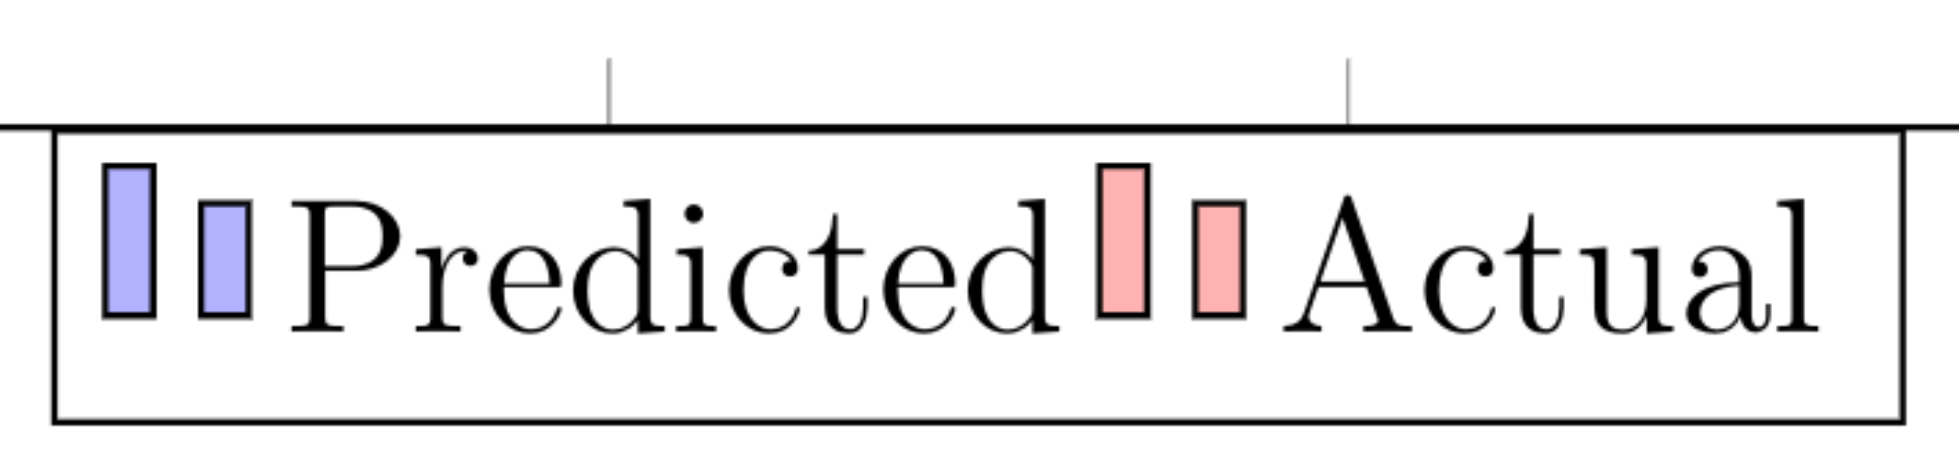
\includegraphics[scale=0.1310]{./figures/legend}}} \end{picture}
    \begin{picture}(0,0) \put(147.35,155.9){\hbox{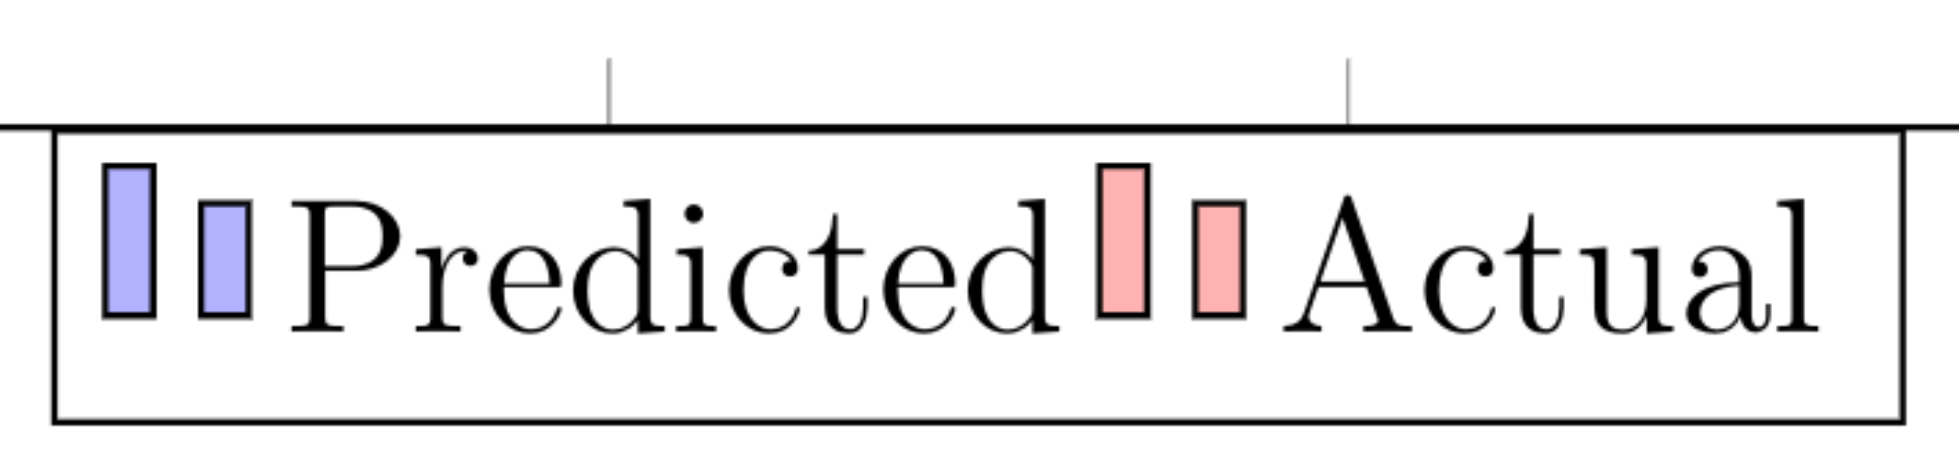
\includegraphics[scale=0.0487]{./figures/legend}}} \end{picture}
    \begin{axis}[
        ybar,
        bar width=.3cm,
        width=0.9\textwidth,
        height=0.45\textwidth,
        symbolic x coords={\texttt{fact}, \texttt{sum\_factors}, \texttt{parse\_files},\texttt{generate\_files},\texttt{add\_footer},\texttt{letter\_count},\texttt{print\_contents},\texttt{count\_vowels},\texttt{separate\_words},\texttt{map\_chars}},
        xtick=data,
        ymode=log,
        ymin=0,ymax=400000,
        xlabel={Programs},
        ylabel={Time (\(\mu s\))},
        xticklabel style={rotate=90},
        tick label style={font=\small},
        xlabel style={yshift=-78pt, font=\large},
        ylabel style={font=\large},
      ]
      \addplot[shift={(2.5,0)}, fill=blue!30!white, error bars/.cd, y dir=both, y explicit] table[x=input_param,y=predicted]{\mydata};
      \addplot[shift={(-2.5,0)}, fill=red!30!white, error bars/.cd, y dir=both, y explicit] table[x=input_param,y=actual, y error plus=actual_order_plus, y error minus=actual_order_minus]{\mydata};
    \end{axis}
  \end{tikzpicture}
  \label{fig:4.1}
  \vspace{-0.5mm}\caption{Comparing \textit{predicted} and \textit{actual runtimes} of Kautuka with 1000 trials --- error bars (unusually) represent one order of magnitude above and below the mean \textit{actual runtime}.}
\end{figure}

\newpage

Measurements were collected on a Dell XPS 15 7590 with the following specifications:

\textbf{Processor} Intel Core i7-9750H CPU @ 2.60GHz × 12

\textbf{Memory} 16 GB 2667 MHz DDR4 RAM

\textbf{OS} Zorin OS 16.2

\textbf{Go Version} go1.19 linux/amd64

The primary source of non-determinism was file-I/O caching. To minimise this effect, we space experiments across set time intervals, separated by redundant operations to clear the cache. These measurements were automated with a bash script, using the Unix \ignore{\texttt{time}} command.

\textbf{Results} In all experiments, our predicted runtime was within an order of magnitude of the true runtime (fig. \hyperref[fig:4.1]{4.1}). One may argue that classifying success as ``within one order of magnitude'' may be too permissive. However, section \hyperref[sec:4.3]{4.3} proves this bound to be sufficiently tight for Kautuka to \textit{consistently outperform} Go. Additionally, there are unpredictable runtime factors (such as caching and inter-process communication) which limit the accuracy of cost analysis.

The programs producing the worst estimates were: \ignore{\texttt{sum\_factors}}, \ignore{\texttt{separate\_words}}, and \ignore{\texttt{map\_chars}}. After investigation, I discovered that the root cause of these inaccuracies were large blocks of non-I/O computations. One explanation for why cost analysis performs worse on these computations is that runtimes of non-I/O operation are orders of magnitude shorter than for I/O operations, measured as a matter of nanoseconds. This requires operations to be executed multiple times in a single run during static profiling, to obtain measurable runtimes. However, repeating operations in such a way makes measurements susceptible to caching effects, reducing the accuracy of static analysis and hence runtime estimates.

However, all other program estimates were accurate, concluding that my \textbf{novel} approach to cost analysis produces \textit{successful} I/O runtime predictions. Since I/O computations dominate runtime in I/O-bound programs (the primary candidates for automatic parallelisation), I constitute this analysis to be a \textit{success}.


\section{Performance on I/O-bound Programs}

\label{sec:4.3}

This section investigates the performance of Kautuka on I/O-bound programs; substantiating claims that Kautuka outperforms Go. Since no existing automatic-parallelisation solutions compile to Go, it would be meaningless to compare their performances with my compiler. Runtime discrepancies would be primarily attributed to the target languages' differing performance, rather than the effectiveness of parallelisation. Thus, the most suitable comparison is with sequential Go, which entails equivalent programming effort to Kautuka (section \hyperref[sec:4.4]{4.4}).

Programmers using the compiler are expected to identify candidate Go files containing expensive (in our case specifically I/O) operations. I performed this methodology on the Kautuka corpus, removing files which fail to satisfy this criteria (\ignore{\texttt{fact}} and \ignore{\texttt{sum\_factors}}). The following benchmarks (fig. \hyperref[fig:4.2]{4.2}) compare the performance of the Kautuka against sequential Go code. By their nature, all chosen Kautuka programs exhibited some degree of parallelisation during execution --- I denote programs containing a combination of both sequential and parallel execution paths with \( \dag \).


\pgfplotstableread[row sep=\\,col sep=&]{
  input_param & kautuka & go & kautuka_err & go_err  \\
  \texttt{parse\_files}\(^\dag\) & 3.93543974 & 6.24607065 & 0.8354047344574917 & 1.4945666661486627\\
  \texttt{generate\_files} & 1.94482751 & 2.65126683 & 0.9112460687334074 & 0.6769222940742172\\
  \texttt{add\_footer}\(^\dag\) & 1.61024851 & 2.5874365499999996 & 1.0762462631630225 & 0.9178685765820006\\
  \texttt{letter\_count} & 1.8470321399999998 & 4.6445662599999995 & 0.6638485104742199 & 1.3971141250272332\\
  \texttt{print\_contents} & 2.3550815299999996 & 3.42348883 & 0.544060833469024 & 0.9825696461239788\\
  \texttt{count\_vowels} & 1.37218422 & 2.52948268 & 0.8774290146103623 & 0.6967561047554715\\
  \texttt{separate\_words} & 5.42705454 & 7.15211727 & 1.0638482023780498 & 1.8217018489778831\\
  \texttt{map\_chars} & 3.04243065 & 4.51591525 & 0.8620350407379548 & 0.931591555199212\\
}\mydata

\begin{figure}[!h]
  \begin{tikzpicture}
    \begin{axis}[
        ybar,
        bar width=.3cm,
        width=0.9\textwidth,
        height=0.45\textwidth,
        symbolic x coords={\texttt{parse\_files}\(^\dag\),\texttt{generate\_files},\texttt{add\_footer}\(^\dag\),\texttt{letter\_count},\texttt{print\_contents},\texttt{count\_vowels},\texttt{separate\_words},\texttt{map\_chars}},
        xtick=data,
        ymin=0,ymax=10,
        xlabel={Programs},
        ylabel={Time (\(s\))},
        xticklabel style={rotate=90},
        tick label style={font=\small},
        xlabel style={yshift=-78pt, font=\large},
        ylabel style={font=\large},
        legend style={at={(0.5,1)},
            anchor=north,legend columns=-1},
      ]
      \addplot[shift={(2.5,0)}, fill=blue!30!white, error bars/.cd, y dir=both, y explicit] table[x=input_param,y=kautuka, y error=kautuka_err]{\mydata};
      \addplot[shift={(-2.5,0)}, fill=red!30!white, error bars/.cd, y dir=both, y explicit] table[x=input_param,y=go, y error=go_err]{\mydata};
      \legend{Kautuka, Go}
    \end{axis}
  \end{tikzpicture}
  \label{fig:4.2}
  \vspace{-0.5mm}\caption{Benchmarking Kautuka against Go. Error bars representing \( \pm \sigma \)}
\end{figure}

\newpage 

\textbf{Results} Our benchmarks show that \textbf{Kautuka consistently outperforms sequential Go}, with performance improvements most pronounced on programs \ignore{\texttt{letter\_count}} and \ignore{\texttt{count\_vowels}}. These programs contain \textit{for-each} loops iterating over file contents, so we deduce that these types of programs exhibit greater performance gains. Overall, these results demonstrate that high-level automatic parallelisation \textit{improves} the performance of I/O-bound programs.


\section{Real-World Compiler Applications}

\label{sec:4.4}

To justify claims that Kautuka integrates into existing workflows, we first illustrate the translation process (from an existing Go file into Kautuka). As is expected with a project of this size, Kautuka lacks some features present in Go such as error handling and file access controls --- which we ignore when translating Go to Kautuka. However, there are no theoretical limitations as to why such features could not be included in the language.

\begin{listing}[!h]
  {
    \captionsetup[figure]{labelformat=empty}%

    \hspace*{-0.5cm}\begin{minipage}{.5\textwidth}
      \begin{minted}{go}
package main 

import ("fmt"; "os") 

func f(x int) {
  for i := 0; i < x; i++ { 
    print(i)
  }
}

func main() { 

  var user_input string 
  fmt.Scan(&user_input)

  user_input_len := len(user_input)

  if user_input_len > 10 { 
    f(user_input_len)
  } else { 
    file, _ := os.OpenFile(user_input,
                           os.O_RDWR, 0777)
    defer file.Close()

    dat, _ := os.ReadFile(file.Name())
    print(string(dat))
  }
}
  \end{minted}
      \begin{center}
        \vspace{-4mm}
        \hspace*{-4mm}{(a) Go}
      \end{center}

      % \label{fig:sample_figure}
    \end{minipage}%
    \begin{minipage}{.5\textwidth}
      \begin{minted}{go}
          package main 
          
          // No explicit imports required 

          func f(x int) {
            for i := 0; i < x; i++ { 
              print(i)
            }
          }
          
          func main() { 

            user_input := input(100) 
            

            user_input_len := len(user_input)

            if user_input_len > 10 { 
              f(user_input_len)
            } else { 
              file := open(user_input)


              
              dat := read(file, 1000)
              print(dat)
            }
          }
      \end{minted}
      \begin{center}
        \vspace{-4mm}
        \hspace*{16mm}{(b) Kautuka}
      \end{center}
    \end{minipage}
  }
  \vspace{2mm}
  \caption{An example I/O-bound program, hand-translated from Go (left) to Kautuka (right).}
  \label{listing:translation}
\end{listing}

\textbf{Results} Listing \hyperref[listing:translation]{1} presents a transliteration of Go to Kautuka with \textit{minimal extra overhead}. Notably, the required annotations (size bounds on I/O inputs) are less strenuous to add than typical parallelisation primitives; the notion of \textit{input sizes} is more grounded than \textit{parallel execution behaviour}, reducing the likelihood of introducing errors. Since Kautuka's syntax is similar to that of Go, and few extra annotations are required, I conclude that Go files can be translated into Kautuka with \textit{minimal effort}.

\newpage 

After translating candidate Go files into Kautuka, the codebase is compiled with my compilation tool. The tool automatically generates parallel Go code from Kautuka files and embeds them into the codebase (deleting Go files once no longer required).

\textbf{Results} Since this tool handles extra complications of a heterogeneous language repository, I conclude that the process of integrating Kautuka into existing Go workflows is \textit{effortless}.

\section{Summary}

\label{sec:4.5}


Kautuka exceeds all success criteria, achieving all core requirements and the majority of extensions listed in Section \hyperref[sec:2.7]{2.7}. Section \hyperref[sec:4.2]{4.2} presents empirical evidence that my novel approach to automatic parallelisation was successful, substantiating the \textit{safety} of side-effect tracking and \textit{accuracy} of cost analysis when implemented in an imperative setting. Our benchmarks reveal that Kautuka outperforms Go on I/O-bound programs (section \hyperref[sec:4.3]{4.3}), highlighting the practicality of high-level automatic parallelisation. Section \hyperref[sec:4.4]{4.4} describes the ease of translating Go files into Kautuka, and how the execution of Kautuka-containing Go codebases requires no additional effort --- showcasing Kautuka's seamless integration into existing workflows.
